\chapter{PAC učenie}

V tejto kapitole sa budeme zaoberať otázkou toho, ako závisí chyba
algoritmu od veľkosti trénovacej množiny. Konkrétne sa budeme
zaoberať otázkami ako:
\begin{itemize}
  \item ``Pri danej veľkosti trénovacej množiny $t$, akú chybu algoritmu
    môžeme očakávať?''
  \item ``Pri danom $t$, s akou pravdepodobnosťou nám algoritmus vráti
    hypotézu, ktorej chyba je menšia ako $\varepsilon$?''
\end{itemize}
Na základe odpovedí na tieto dve otázky potom budeme schopní zodpovedať
nasledovné, príbuzné otázky:
\begin{itemize}
  \item ``Akú veľkú trénovaciu množinu máme zvoliť, aby sme dosiahli
    dostatočne malú ($\leq \epsilon$) chybu algoritmu?''
  \item ``Aké $t$ máme zvoliť, aby sme s vysokou pravdepodobnosťou
    ($\geq \delta$) dostali dostatočne dobrú ($\leq \varepsilon$)
    hypotézu?''
\end{itemize}

Odtiaľ sa odvíja názov \emph{PAC učenie} (z anglického
\emph{probably approximately correct learning}).

Obe typy ``chýb'' sú potrebné, keď sa chceme rozprávať o tom,
aký vplyv má veľkosť trénovacej množiny na trénovací algoritmus.
Po prvé, $\varepsilon$ je potrebné ako miera toho, čo je dostatočne
dobrá hypotéza. Po druhé, $\delta$ je potrebné, nakoľko vo všeobecnosti
nevieme garantovať, že dostaneme dobrú hypotézu: mohli sme si
(s malou pravdepodobnosťou) vytiahnuť zlé trénovacie dáta.

Začneme definíciou PAC učenia, ktorá ešte nebude brať do úvahy
výpočtovú stránku učenia.

Zameriame sa na binárne klasifikačné úlohy, v ktorých je cieľom rozlíšiť medzi
reprezentantmi nejakého cieľového konceptu od nereprezentantov. Napríklad
cieľovým konceptom môže byť ``písmeno A''. Hypotéza dostane na vstupe
obrázok $32 \times 32$ a má povedať, či tento obrázok vyobrazuje
písmeno A alebo nie.

Máme teda množinu konceptov $C$, z ktorej pochádza cieľový koncept $c$.
Náš trénovací algoritmus ale nevie, ktorý z nich to je. Jeho úlohou je
nájsť dobrú aproximáciu, ktorú bude hľadať v množine hypotéz $H$. Budeme
predpokladať, že $H \supseteq C$, aby bolo zaručená existencia dobrej
hypotézy.

Algoritmus na vstupe dostane niekoľko trénovacích príkladov v tvare dvojíc
$(x, c(x))$, pričom $x$ pochádza z pravdepodobnostného rozdelenia $P$.
Uvažovať $y$ v rozdelení $P$ nie je potrebné, nakoľko je jednoznačne
určené cez $x$ a $c$.

\begin{definition}
  Nech $C$ je množina konceptov nad množinou vstupov $X$. Hovoríme, že
  $C$ je \emph{PAC naučiteľná} ak existuje algoritmus $L$ s nasledujúcou
  vlastnosťou: pre každý (cieľový) koncept $c \in C$, pre každé
  $\varepsilon > 0$, $\delta > 0$ a pre každé možné pravdepodobnostné
  rozdelenie $P$, ak algoritmu $L$ dáme na vstupe $t$ trénovacích
  príkladov $(x_i, c(x_i))$ náhodne vybraných podľa $P$ a $t$ je
  dostatočne veľké, tak nám algoritmus s pravdepodobnosťou nanajvýš
  $\delta$ vráti hypotézu $\hat{h} \in C$ spĺňajúcu $\err(\hat{h}) \leq \varepsilon$.
  Táto pravdepodobnosť sa berie cez náhodnosť v ťahaní trénovacích
  príkladov a prípadnú náhodnosť algoritmu $L$.
\end{definition}
\begin{remark}
  Neskôr túto definíciu rozšírime tak, aby brala do úvahy aj výpočtovú
  stránku algoritmu. Vtedy sa budeme zaoberať aj tým, v akom čase náš
  algoritmus beží a koľko trénovacích príkladov potrebuje. Budeme
  hovoriť o \emph{efektívnej PAC naučiteľnosti}.
\end{remark}
\begin{remark}
  Pripomíname, že chyba hypotézy $h$ sa pre klasifikačné úlohy počíta
  ako
  $$\err(h) = \E_{x \sim P} \left[ h(x) \neq c(x) \right] = \prob_{x \sim P}( h(x) \neq c(x) ).$$
\end{remark}

Budeme hovoriť, že trénovací príklad $(x, y)$ je \emph{pozitívny},
ak $y = 1$. V opačnom prípade budeme hovoriť, že príklad je
\emph{negatívny}.




\section{Konečné množiny hypotéz}

V tejto časti sa zameriame na konečné množiny hypotéz.

Budeme predpokladať, že algoritmus vždy vráti \emph{konzistentný
klasifikátor}: takú hypotézu, ktorá je konzistentná s trénovacími
príkladmi, teda že pre ľubovoľnú trénovaciu množinu $T$ platí
$\err_T(\hat{h}) = 0$. Za predpokladu $H \supseteq C$ je to
splniteľný predpoklad: jedným konzistentným klasifikátorom je
samotný cieľový koncept $c$.



\subsection{Základné výsledky}

\begin{theorem} \label{thm:badhypobound}
  Nech je dané $\varepsilon > 0$. Hypotézu nazveme \emph{zlú}, ak jej
  chybovosť je väčšia ako $\varepsilon$. Potom vieme pomocou počtu
  trénovacích príkladov $t$ odhadnúť pravdepodobnosť, že nám algoritmus
  vráti zlú hypotézu, nasledovne:
  $$\prob(\err(\hat{h}) > \varepsilon) < |H| \cdot e^{-\varepsilon t}$$
\end{theorem}
\begin{proof}
  Ak žiadna zlá hypotéza nie je konzistentná s príkladmi, tak výstupom
  algoritmu nemôže byť zlá hypotéza. Budeme sa teda snažiť zhora odhadnúť
  pravdepodobnosť, že aspoň jedna zlá hypotéza ``prežila''.
  
  Nech $h$ je ľubovoľná zlá hypotéza. Pravdepodobnosť, že je konzistentná
  s trénovacími príkladmi, je rovná $(1 - \err(h))^t$, čo vieme odhadnúť
  nasledovne:
  $$(1 - \err(h))^t < (1 - \varepsilon)^t \leq e^{-\varepsilon t}$$
  
  Zlých hypotéz je nanajvýš toľko, koľko je všetkých hypotéz, teda
  $|H|$. Pravdepodobnosť, že aspoň jedna z nich bude konzistentná s
  príkladmi, sa dá odhadnúť zhora ako súčet ich pravdepodobností:
  $$\prob(\text{aspoň jedna zlá}) < |H| \cdot e^{-\varepsilon t}$$
  Odkiaľ dostávame požadovanú nerovnosť.
\end{proof}
\begin{remark}
  Vo vyššie uvedenom dôkaze sme nepredpokladali nič o pravdepodobnostnom
  rozdelení $P$ ani o cieľovom koncepte $c$. Uvedená veta teda platí
  pre ľubovoľné $P$ a $c$.
\end{remark}

Čo ak nás zaujíma druhá otázka: ``Ako závisí chyba algoritmu od počtu
trénovacích príkladov?'' Pri klasifikačných úlohách je táto otázka úzko
spätá s predošlou otázkou, kde sme sa zaujímali o $\varepsilon$ a $\delta$.

\begin{theorem}
  Platí
  $$ \chalg \leq \frac{1}{t} \cdot \left( \ln{|H|} + \ln{t} + 1 \right). $$
\end{theorem}
\begin{proof}
  Ak nám algoritmus vráti dobrú hypotézu (s chybou nanajvýš $\varepsilon$),
  vieme jej chybu odhadnúť zhora ako $\varepsilon$. Ak nám algoritmus vráti
  zlú hypotézu, jej chyba je nanajvýš $1$. Z toho dostávame nasledovný
  horný odhad na celkovú chybu algoritmu:
  $$ \chalg = \E \left[ \err(\hat{h}) \right] \leq \prob(\err(\hat{h}) \leq \varepsilon) \cdot \varepsilon + \prob(\err(\hat{h}) > \varepsilon) \cdot 1$$
  Pritom pravdepodobnosti na pravej strane vieme odhadnúť zhora:
  $\prob(\err(\hat{h}) \leq \varepsilon) \leq 1$, a druhú vieme
  odhadnúť pomocou vety \ref{thm:badhypobound}. Dostávame tak odhad
  $$ \chalg \leq 1 \cdot \varepsilon + |H| \cdot e^{-\varepsilon t}. $$
  My sme si ale mohli zvoliť $\varepsilon$ ľubovoľne. Ak teda chceme
  dostať čo najlepší odhad, nájdeme $\varepsilon$, pre ktoré je výraz
  na pravej strane čo najmenší. Zderivujme a položme rovné nule:
  \begin{align}
    1 - |H| \cdot t \cdot e^{-\varepsilon t} &= 0 \\
    \varepsilon &= \frac{1}{t} \cdot \left( \ln{|H|} + \ln{t} \right)
  \end{align}
  Odtiaľ dosadením dostaneme požadovaný odhad na chybu algoritmu.
\end{proof}

Na základe týchto dvoch viet vieme sformulovať postačujúce podmienky
na $t$ také, aby boli príslušné chyby ($\varepsilon, \delta$ a chyba
algoritmu) dostatočne malé. Sformulujeme a dokážeme jednu z nich.

\begin{corollary}
  Množina hypotéz $H$ je PAC-naučiteľná: pre každé $\varepsilon > 0$,
  $\delta > 0$, ľubovoľné pravdepodobnostné rozdelenie $P$ a ľubovoľný
  cieľový koncept $f \in H$ existuje počet trénovacích príkladov $t$
  taký, že platí
  $$\prob(\err(\hat{h}) \leq \varepsilon) \geq 1 - \delta.$$
  Ekvivalentne,
  $$\prob(\err(\hat{h}) > \varepsilon) \leq \delta.$$
\end{corollary}
\begin{proof}
  Podľa vety \ref{thm:badhypobound} platí
  $$\prob(\err(\hat{h}) > \varepsilon) < |H| \cdot e^{-\varepsilon t}.$$
  Stačí nám teda zvoliť také $t$, aby bol výraz na pravej strane menší
  rovný $\delta$. Odtiaľ dostaneme postačujúci počet trénovacích
  príkladov $t$:
  \begin{align}
    |H| \cdot e^{-\varepsilon t} &\leq \delta \\
    \ln{|H|} - \varepsilon t &\leq \ln{\delta} \\
    \varepsilon t &\geq \ln{|H|} - \ln{\delta} \\
    t &\geq \frac{1}{\varepsilon} \cdot \left( \ln{|H|} + \ln{\frac{1}{\delta}} \right)
  \end{align}
\end{proof}



\subsection{Problém konjunkcie}

Jedným príkladom problému, kde je množina hypotéz konečná, je
\emph{problém konjunkcie pozitívnych literálov}. Na ňom si ukážeme,
že (aspoň v niektorých problémoch) sú vyššie uvedené odhady relatívne
tesné.

Nech je dané $n$. Množina vstupov sú všetky možné ohodnotenia boolovských
premenných $x_1, \ldots, x_n$. Napríklad $x_1 = 0$, $x_2 = 1$, $x_3 = 0$
je priradenie hodnôt. Priradenia vieme zapísať vo vektorovom tvare:
vyššie uvedený príklad by sme zapísali ako $x = (0, 1, 0)$. Všetkých
vstupov je zrejme $2^n$.

Množina konceptov $C$ sú všetky konjunkcie nad pozitívnymi literálmi
$x_1, \ldots, x_n$. Tieto konjunkcie sú chápané ako funkcie, ktoré
vracajú $1$ iba ak dané ohodnotenie premenných spĺňa túto konjunkciu.
Napríklad $x_1 \land x_3 \land x_4$ vráti $1$ na všetkých tých vstupoch,
kde táto konjunkcia platí: musí platiť $x_1 = 1$, $x_3 = 1$, $x_4 = 1$,
ale ostatné premenné už môžu mať ľubovoľnú hodnotu. Všetkých konceptov
je zrejme tiež $2^n$. Množina hypotéz $H$ bude rovnaká, ako množina
konceptov.

Aby sme videli, že konzistentnosť s trénovacími príkladmi je realistická
požiadavka, ukážeme si, ako sa dá na základe trénovacích príkladov
zostrojiť nejaký konzistentný klasifikátor.
\begin{theorem}
  Nech hypotéza $\hat{h}$ je konjunkciou všetkých tých premenných, ktoré
  sa vyskytujú vo všetkých pozitívnych trénovacích príkladoch. Potom
  $\hat{h}$ je konzistentná so všetkými trénovacími príkladmi.
\end{theorem}
\begin{proof}
  Ak $(x, y)$ je pozitívny príklad, v cieľovej hypotéze $c$ môžu byť
  jedine tie premenné, ktoré majú v $x$ priradenú hodnotu $1$. Keď
  túto úvahu zopakujeme pre všetky pozitívne príklady, dostaneme
  niekoľko množín ``povolených premenných''. Cieľová premenná musí byť
  podmnožinou všetkých z nich, teda je podmnožinou ich prieniku. Pritom
  ich prienik je práve hypotéza $\hat{h}$.
  
  Z toho vyplýva, že ak nie je splnené $c$, nemôže byť splnené ani $h$.
  Naša hypotéza totiž kladie ešte väčšie požiadavky na hodnoty
  premenných. Teda,
  $$(c(x) = 0) \implies (h(x) = 0),$$
  takže $h$ je konzistentná s negatívnymi príkladmi.
  
  Čo sa týka pozitívnych príkladov, v $h$ sú všetky tie premenné, ktoré
  sme do nej mohli dať tak, aby bola konzistentná so všetkými pozitívnymi
  príkladmi. Teda jej konzistentnosť s pozitívnymi príkladmi vyplýva
  priamo z jej konštrukcie.
\end{proof}

Uvedieme teraz niektoré výsledky z predchádzajúcej časti tak, ako platia
pre problém konjunkcie.

\begin{corollary}
  Platí
  $$ \chalg \leq \frac{1}{t} \cdot \left( n \ln{2} + \ln{t} + 1 \right) = O\left( \frac{n + \ln{t}}{t} \right). $$
\end{corollary}
\begin{corollary} \label{cor:mconj_de}
  Aby sme mali zaručené (s pravdepodobnosťou aspoň $1 - \delta$), že
  dostaneme hypotézu s chybou nanajvýš $\varepsilon$, stačí zvoliť
  veľkosť trénovacej množiny nasledovne:
  $$ t \geq \frac{1}{\varepsilon} \cdot \left( n \ln{2} + \ln{\frac{1}{\delta}} \right) = \Omega\left( \frac{n + \ln{\frac{1}{\delta}}}{\varepsilon} \right) $$
\end{corollary}

Tieto odhady sú relatívne tesné. Vo všeobecnom prípade je ťažké dostať
nejaký dolný odhad, nakoľko pravdepodobnostné rozdelenie $P$ a cieľový
koncept $c$ môžu byť degenerované a ``uľahčiť algoritmu robotu''.
Uvidíme ale, že pre niektoré ``ťažké'' prípady vieme spraviť dolný odhad.

\begin{theorem} \label{thm:mconj_lb}
  Existuje pravdepodobnostné rozdelenie $P$ a cieľový koncept $c \in C$
  také, že nech je trénovací algoritmus ľubovoľný, pre jeho chybu platí
  nasledovný dolný odhad:
  $$ \chalg \geq \frac{1}{2e} \cdot \frac{n-1}{t+1} = \Omega \left( \frac{n}{t} \right)$$
\end{theorem}

V znení vety je trochu obmedzujúce, že cieľový koncept musí byť
pevne vybraný. Ukážeme teda najprv, že pokiaľ tvrdenie dokážeme
pre náhodne vybrané $c$, bude z neho plynúť pôvodné tvrdenie.

\begin{lemma}
  Nech $P_C$ je pravdepodobnostné rozdelenie nad množinou konceptov $C$.
  Cieľovú hypotézu vyberieme náhodne podľa $P_C$. Ak pre nejaké číslo
  $k$ platí, že stredná hodnota chyby algoritmu je aspoň $k$, tj.
  $$\E_{c \sim P_C} \left[ \chalg \right] \geq k,$$
  tak existuje voľba cieľového konceptu $c \in C$ taká, že chyba
  algoritmu bude tiež aspoň $k$.
\end{lemma}
\begin{proof}
  Ak by na každom cieľovom koncepte bola chyba algoritmu menšia ako $k$,
  potom by aj ľubovoľný vážený priemer chýb (zodpovedajúci strednej
  hodnote s rozdelením $P_C$) bol menší ako $k$. To by bol spor.
\end{proof}

Ďalej pokračujeme dôkazom vety \ref{thm:mconj_lb}. V ňom si už môžeme
dovoliť vyberať cieľový koncept náhodne.

\begin{proof}
  Zvolíme pravdepodobnostné rozdelenie, ktoré priradí nenulovú
  pravdepodobnosť iba nasledovnej sade vstupov. Konkrétne
  pravdepodobnosti určíme neskôr v dôkaze tak, ako sa nám to bude hodiť.
  \begin{align}
    x^{(1)} &= (0, 1, 1, \ldots, 1, 1) \\
    x^{(2)} &= (1, 0, 1, \ldots, 1, 1) \\
            &\vdots \\
    x^{(n)} &= (1, 1, 1, \ldots, 1, 0)
  \end{align}
  Tieto vstupy majú nasledujúcu vlastnosť. Pre ľubovoľný koncept $c$
  platí, že sa v ňom nachádza konjunkcia $x_i$ vtedy a len vtedy, keď
  $f(x^{(i)}) = 0$. Každý z týchto vstupov sa dá teda chápať ako
  ``test na niektorú premennú''.
  
  Trénovacie príklady potom môžeme chápať tak, že algoritmu dávajú
  informáciu o jednotlivých premenných: ``Je alebo nie je v cieľovej
  hypotéze?'' Pokiaľ ale niektorý zo vstupov $x^{(i)}$ nie je medzi
  trénovacími príkladmi, nemáme žiadnu informáciu o tom, či sa tam
  príslušná premenná nachádza. Ak si potom $\hat{h}$ vytiahne pri
  testovaní takýto vstup, môže jedine hádať, aká je správna odpoveď.
  Šanca úspechu pri hádaní bude $\frac{1}{2}$, pokiaľ vyberieme $c$
  rovnomerne náhodne z celej množiny konceptov.
  
  Označme si pravdepodobnosti pridelené jednotlivým vstupom $p_1, \ldots, p_n$.
  Aká je šanca, že pri trénovaní vstup $x^{(i)}$ nedostaneme a potom si ho
  pri testovaní vytiahneme?
  $$p_i \cdot (1 - p_i)^t$$
  Celková pravdepodobnosť, že si vytiahneme pri testovaní vstup mimo
  trénovacej množiny, je potom súčet jednotlivých pravdepodobností
  (nakoľko sú jednotlivé udalosti dizjunktné):
  $$\sum_{i=1}^n p_i \cdot (1 - p_i)^t$$
  V týchto prípadoch bude mať $\hat{h}$ chybu $\frac{1}{2}$. V ostatných
  prípadoch sme si vytiahli počas testovania nejaký príklad, ktorý bol aj
  v trénovacej množine. Pokiaľ sme si ho zapamätali, tak budeme mať chybu
  $0$, v každom prípade bude ale chyba aspoň $0$. Dostávame tak nasledovný
  dolný odhad na chybu algoritmu:
  $$ \E_{c \in C} \left[ \chalg \right] \geq \frac{1}{2} \cdot \left( \sum_{i=1}^n p_i \cdot (1 - p_i)^t \right) $$
  
  Ako ale zvoliť $p_1, \ldots, p_n$ tak, aby sme dostali dobrý dolný
  odhad? Skúsime zvoliť $p_i$ také, pre ktoré nadobúda výraz
  $p_i \cdot (1 - p_i)^t$ maximum. Zderivovaním a položením rovné
  $0$ dostaneme
  $$p_i = \frac{1}{t+1}.$$
  Pokiaľ ale $t \neq n - 1$, nemôžeme zvoliť všetky pravdepodobnosti
  takéto: pre $t < n - 1$ je súčet pravdepodobností priveľký a pre $t > n - 1$
  primalý. Prvý prípad nás nezaujíma, nakoľko je to ``len konštanta''
  (v zmysle $t \to \infty$). V druhom prípade si vieme zvoliť jedného
  ``obetného baránka'' $p_1$, ktorému priradíme celú zvyšnú
  pravdepodobnosť.
  \begin{align}
    p_1 &= 1 - \frac{n-1}{t+1} \\
    p_2 &= \frac{1}{t+1} \\
        &\vdots \\
    p_n &= \frac{1}{t+1}
  \end{align}
  Dosadíme a dostaneme tak odhad:
  $$ \E_{c \in C} \left[ \chalg \right] \geq \frac{1}{2} \cdot \left( (n - 1) \cdot \frac{1}{t+1} \cdot \left( 1 - \frac{1}{t+1} \right)^t + \frac{n-1}{t+1} \cdot \left( 1 - \frac{n-1}{t+1} \right)^t   \right) $$
  Odignorujeme druhý sčítanec, čím sa nám výraz na pravej strane môže
  len zmenšiť, takže nerovnosť sa zachová. Ďalej použijeme odhad
  $$ \left( 1 - \frac{1}{t+1} \right)^t \geq \frac{1}{e}, $$
  ktorý platí pre všetky prirodzené $t$. (Tento odhad sa dá dokázať
  napríklad tak, že sa dokáže, že daný výraz je rastúci od $t$. Odhad
  z toho už plynie ľahko, nakoľko jeho limita pre $t \to \infty$ je
  práve $\frac{1}{e}$.) Dostaneme tak požadovanú nerovnosť:
  $$ \E_{c \in C} \left[ \chalg \right] \geq \frac{1}{2e} \cdot \frac{n-1}{t+1} $$
\end{proof}

Dolný odhad zodpovedajúci dôsledku \ref{cor:mconj_de} uvedieme bez dôkazu.

\begin{theorem}
  Pre ľubovoľný trénovací algoritmus existuje pravdepodobnostné rozdelenie
  $P$ a cieľová hypotéza $f \in H$, ktoré vynútia, že algoritmus bude
  potrebovať aspoň
  $$ t = \Omega \left( \frac{1}{\varepsilon} \cdot \left( n + \ln{\frac{1}{\delta}} \right) \right), $$
  aby platilo
  $$ \prob(\err(\hat{h}) > \varepsilon) \leq \delta.$$
\end{theorem}

\TODO{dôkaz}




\section{Nekonečné množiny hypotéz}

Vyššie uvedený postupy pre konečné množiny hypotéz zlyhajú, ak
$|H| = \infty$: nedostaneme z nich žiaden odhad. Aj pre nekonečné
množiny hypotéz je ale možné odvodiť horné odhady, ktoré sa už nebudú
odvíjať od veľkosti množiny $H$, ale od nejakej jej miery zložitosti.
Touto mierou zložitosti bude tzv. \emph{Vapnik-Chervonenkisova dimenzia}.
Predtým sa ale pozrieme na jednoduchý príklad.




\subsection{Obdĺžniková hra}

Ide o klasifikačnú úlohu. Množina vstupov sú všetky body v rovine.
Množina konceptov sú všetky obdĺžniky, ktorých strany sú rovnobežné
so súradnicovými osami. Pre každý bod v rovine sa teda pýtame, či je
vo vnútri cieľového obdĺžnika $c$ alebo nie. Body na okraji obdĺžnika
považujeme, že sú vnútri.

Pre jednoduchosť argumentu použijeme konkrétny trénovací algoritmus.
Dôkaz by sa dal zovšeobecniť na prípad, kedy jediné, čo o algoritme
predpokladáme je, že nám vracia konzistentný klasifikátor. S nasledovným
konzistentným klasifikátorom to ale bude jednoduchšie.

\medskip

Z trénovacích príkladov vezmime tie pozitívne. Ako hypotézu $\hat{h}$
zvolíme najmenší (vzhľadom na inklúziu) osovorovnobežný obdĺžnik,
ktorý obsahuje všetky body vo vybraných príkladoch. Na obrázku
\ref{rectgame:hath} ilustrujeme konštrukciu $\hat{h}$ a porovnávame
ho s $c$.

\TODO{obrázok}

\begin{lemma}
  Každá množina bodov $(x_1, y_1), \ldots, (x_t, y_t)$ má unikátny
  \emph{bounding box}: najmenší (vzhľadom na inklúziu) osovorovnobežný
  obdĺžnik, ktorý ich všetky obsahuje.
\end{lemma}
\begin{proof}
  Každý obdĺžnik je jednoznačne určený $x$-ovými súradnicami ľavého
  a pravého okraja a $y$-ovými súradnicami dolného a horného okraja.
  Označme ich $x_\larr, x_\rarr$ a $y_\darr, y_\uarr$.
  Vo vnútri sú práve tie body $(x, y)$, ktoré spĺňajú
  $$x_\larr \leq x \leq x_\rarr,\ y_\darr \leq y \leq y_\uarr.$$
  Ak teda majú byť všetky spomínané body vo vnútri, musí platiť
  $$
    x_\larr \leq \min x_i,\ 
    x_\rarr \geq \max x_i,\ 
    y_\darr \leq \min y_i,\ 
    y_\uarr \geq \max y_i
  $$
  Najmenší osovorovnobežný obdĺžnik, ktorý toto spĺňa, je ten, pre
  ktorý nastávajú v jednotlivých nerovnostiach rovnosti. Teda
  $x_\larr = \min x_i$, $x_\rarr = \max x_i$, $y_\darr = \min y_i$ a $y_\uarr = \max y_i$.
\end{proof}
\begin{corollary}
  Obdĺžnik $\hat{h}$ je podmnožinou cieľového obdĺžnika $c$.
\end{corollary}
\begin{corollary}
  Obdĺžnik $\hat{h}$ je konzistentný klasifikátor.
\end{corollary}
\begin{proof}
  Konzistentnosť na pozitívnych príkladoch vyplýva z konštrukcie $\hat{h}$.
  Každý negatívny príklad je mimo $c$ a teda aj mimo $\hat{h}$, je teda
  konzistentný aj s negatívnymi príkladmi.
\end{proof}

\begin{theorem}
  Obdĺžniková hra je PAC naučiteľná: pre každý cieľový obdĺžnik $c \in C$,
  $\varepsilon > 0$, $\delta > 0$ a pravdepodobnostné rozdelenie $P$, ak
  vyššie popísanému algoritmu dáme $t$ trénovacích príkladov z $P$ a
  platí
  $$ t \geq \frac{4}{\varepsilon} \cdot \ln{\frac{4}{\delta}}, $$
  tak nám algoritmus s vysokou pravdepodobnosťou vráti hypotézu s nízkou
  chybou:
  $$ \prob(\err(\hat{h}) > \varepsilon) \leq \delta. $$
\end{theorem}
\begin{proof}
  Zle klasifikované body sú práve tie, ktoré sú vo vnútri $c$ ale nie sú
  vo vnútri $\hat{h}$. Každý z týchto bodov padne do aspoň jedného
  z okrajových ``pásikov'' (nerátajúc jeden z okrajov), ako je
  zobrazené na obrázku \ref{rectgame:strips}.
  
  Pod \emph{váhou} množiny budeme rozumieť pravdepodobnosť, že náhodný
  bod z rozdelenia $P$ padne do tejto množiny.
  Označme $p_\larr, p_\rarr, p_\uarr, p_\darr$ postupne váhy ľavého,
  pravého, horného, resp. dolného pásika. Chyba $\hat{h}$ sa dá zhora
  odhadnúť ako súčet týchto váh:
  $$ \err(\hat{h}) \leq p_\larr + p_\rarr + p_\uarr + p_\darr. $$
  
  Ak by sme voľbou dostatočne veľkého $t$ vedeli zaručiť
  (s pravdepodobnosťou aspoň $1 - \delta$), že dostaneme takú hypotézu
  $\hat{h}$, pre ktorú je výraz na pravej strane nanajvýš $\varepsilon$,
  vyhrali by sme. Ukážeme, že vieme zaručiť
  $$ p_\larr, p_\rarr, p_\uarr, p_\darr \leq \frac{\varepsilon}{4}. $$
  Postup bude vo všetkých štyroch prípadoch ten istý, ukážeme si to
  teda len na ľavom pásiku.
  
  \TODO{dôkaz (eww, grc)}
\end{proof}




\subsection{Vapnik-Chervonenkisova dimenzia}

Vapnik-Chervonenkisova dimenzia (alebo skrátene VC dimenzia) je miera
zložitosti množiny hypotéz, pomocou ktorej sme schopní tvoriť tvrdenia
v štýle PAC učenia. Na jej definíciu budeme potrebovať niekoľko pomocných
pojmov.

\begin{definition}
  Majme konečnú podmnožinu vstupov $S \subseteq X$. Hovoríme, že množina
  hypotéz $H$ \emph{rozbíja} množinu $S$, ak platí: nech označíme vstupy
  v $S$ ako pozitívne alebo negatívne akokoľvek, v množine $H$ existuje
  hypotéza konzistentná s týmto označením.
\end{definition}

Intuitívne, množina $S$ je rozbitá hypotézami $H$, ak nie je pre
hypotézy v $H$ príliš náročné modelovať príklady v $S$: sú schopné
ich modelovať akokoľvek.

\begin{definition}
  Vapnik-Chervonenkisova dimenzia množiny hypotéz $H$, označovaná
  $VCD(H)$, je veľkosť najväčšej množiny $S \subseteq X$, ktorá
  sa dá rozbiť hypotézami v $H$. Ak sa dá rozbiť ľubovoľne veľká
  množina $S$, definujeme $VCD(H) = \infty$.
\end{definition}

Teda na to, aby sme ukázali dolný odhad $VCD(H) \geq d$, stačí nám
nájsť jednu množinu $S$ veľkosti $d$, ktorá sa dá rozbiť. Aby sme ale
ukázali horný odhad $VCD(H) \leq d$, musíme ukázať, že žiadna množina
veľkosti $d + 1$ sa nedá rozbiť: teda že existuje také označenie vstupov,
pre ktoré neexistuje v $H$ konzistentný klasifikátor. Z tohto dôvodu je
obvykle ťažšie dokázať horný odhad na VC dimenziu, ako dolný odhad.

\begin{lemma}
  Majme dve množiny hypotéz $H$ a $H'$ nad tou istou množinou vstupov $x$.
  Ak platí $H \supseteq H'$, tak potom platí $VCD(H) \succeq VCD(H')$ (kde
  $\succeq$ je relácia $\geq$ prirodzene rozšírená na $\nats \cup \{ \infty \}$).
\end{lemma}
\begin{proof}
  Ak sa množina $S$ dá rozbiť pomocou $H'$, potom, pretože každá hypotéza
  v $H'$ je aj v $H$, dá sa táto množina rozbiť aj pomocou $H$ (rovnakým
  spôsobom).
\end{proof}

Než uvedieme vety hovoriace o PAC naučiteľnosti, uvedieme príklady
niektorých nekonečných množín hypotéz, a neformálne zdôvodníme ich
VC dimenzie. Väčšinou budú geometrického charakteru (čo je prirodzené,
ak máme mať nekonečnú množinu hypotéz).

\paragraph{Intervaly na reálnych číslach.} Nie je ťažké vidieť, že
ľubovoľná dvojica bodov sa dá rozbiť. Na druhej strane, ak máme tri
body, tak ich vieme označiť ako na obrázku \ref{vc:interval}, čo nie
je konzistentné so žiadnym intervalom. Takže VC dimenzia je $2$.

\begin{figure}
  \centering
  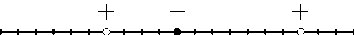
\includegraphics[scale=1]{obrazky/interval.pdf}
  \caption{Žiaden interval nevytvorí takéto označenie bodov.}
  \label{vc:interval}
\end{figure}

\paragraph{Polroviny v rovine.} Každá trojica bodov tvoriacich
nedegenerovaný trojuholník sa dá rozbiť, ako je ilustrované na
obrázku \ref{vc:halfplane}. Na druhej strane, žiadna štvorica bodov
sa rozbiť nedá: ak tvoria konvexný štvoruholník, tak jednu protiľahlú 
dvojicu označíme kladne a druhú záporne. Ak tvoria nekonvexný 
štvoruholník, jeden z bodov je vo vnútri trojuholníka tvoreného 
ostatnými tromi: tento bod označíme kladne a ostatné body záporne.
Takže VC dimenzia je $3$.

\begin{figure}
  \centering
  \begin{subfigure}[b]{0.3\linewidth}
    \centering
    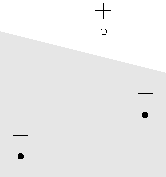
\includegraphics[scale=1]{obrazky/halfplane1.pdf}
    \caption{}
  \end{subfigure}
  ~
  \begin{subfigure}[b]{0.3\linewidth}
    \centering
    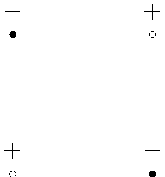
\includegraphics[scale=1]{obrazky/halfplane2.pdf}
    \caption{}
  \end{subfigure}
  ~
  \begin{subfigure}[b]{0.3\linewidth}
    \centering
    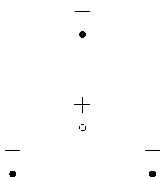
\includegraphics[scale=1]{obrazky/halfplane3.pdf}
    \caption{}
  \end{subfigure}
  \caption{Polroviny v rovine. V situácii (a) vieme nájsť deliacu priamku, v (b) a (c) nie.}
  \label{vc:halfplane}
\end{figure}

\paragraph{Osovorovnobežné obdĺžniky.} Štvorica bodov, ktorá sa dá
rozbiť, je ilustrovaná na obrázku \ref{vc:rect}, nie každá štvorica
bodov sa ale dá rozbiť. Na druhej strane, žiadna pätica bodov sa nedá
rozbiť. Rozoberieme dva prípady: ak je aspoň jeden z bodov vo vnútri 
bounding boxu (nie na okraji), tak ho označíme záporne a všetky body na 
okraji kladne. Ak sú všetky body na obvode bounding boxu, na jednej 
strane toho obdĺžnika musia ležať aspoň dva body. Jeden z nich označíme 
kladne a druhý záporne. Takže VC dimenzia je $4$.

\begin{figure}
  \centering
  \begin{subfigure}[b]{0.23\linewidth}
    \centering
    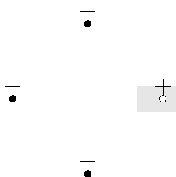
\includegraphics[scale=1]{obrazky/vc_rect1.pdf}
    \caption{}
  \end{subfigure}
  ~
  \centering
  \begin{subfigure}[b]{0.23\linewidth}
    \centering
    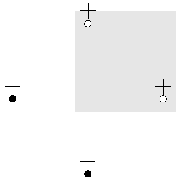
\includegraphics[scale=1]{obrazky/vc_rect2.pdf}
    \caption{}
  \end{subfigure}
  ~
  \centering
  \begin{subfigure}[b]{0.23\linewidth}
    \centering
    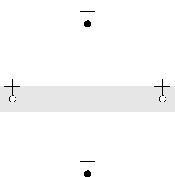
\includegraphics[scale=1]{obrazky/vc_rect3.pdf}
    \caption{}
  \end{subfigure}
  ~
  \centering
  \begin{subfigure}[b]{0.23\linewidth}
    \centering
    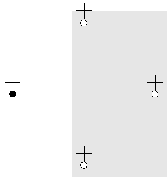
\includegraphics[scale=1]{obrazky/vc_rect4.pdf}
    \caption{}
  \end{subfigure}
  \caption{Osovorovnobežné obdĺžniky. Štvorica bodov, ktorá sa dá rozbiť.
    Jednotlivé obrázky zobrazujú všetky netriviálne označenia bodov a
    príslušné konzistentné klasifikátory.}
  \label{vc:rect}
\end{figure}

\medskip

Nakoniec hlavný výsledok, kvôli ktorému je VC dimenzia zaujímavá.

\begin{theorem}[Blumer et. al., 1989 \cite{blumer1989learnability}]
  Nech $C$ je ľubovoľná množina konceptov. Nech $H$ je množina hypotéz
  s VC dimenziou rovnou $d$. Nech $L$ je ľubovoľný algoritmus, ktorý
  pre ľubovoľnú sadu $t$ trénovacích príkladov vráti hypotézu $\hat{h}$
  konzistentnú s príkladmi. Potom $L$ je PAC trénovací algoritmus pre
  množinu konceptov $C$ s použitím hypotéz v $H$, pokiaľ je $t$
  dostatočne veľké:
  $$ t \geq c_0 \left( \frac{1}{\varepsilon} \ln{\frac{1}{\delta}} + \frac{d}{\varepsilon} \ln{\frac{1}{\varepsilon}} \right) $$
  pre nejakú konštantu $c_0 > 0$.
\end{theorem}

\TODO{dôkaz}

\begin{theorem}[Haussler et. al., 1994 \cite{haussler1994predicting}]
  Ak VC dimenzia je $d$, tak ľubovoľný trénovací algoritmus, ktorý vždy
  vracia hypotézy konzistentné s trénovacími príkladmi, má chybu nanajvýš
  $$ \E \left[ \err(\hat{h}) \right] = O\left( \frac{d}{t} \ln{\frac{t}{d}} \right). $$
\end{theorem}

\TODO{dôkaz}

Čo ale v prípade, že neexistuje konzistentný klasifikátor? Taká situácia
nastane, keď buď cieľový koncept nie je v množine hypotéz, alebo keď v
probléme vystupuje šum. Ukazuje sa, že aj v takom prípade sa dá
odhadnúť chyba hypotézy.

\begin{theorem}[Vapnik \& Chervonenkis, 1971 \cite{chervonenkis1971theory}]
  Nech $h^\star$ je hypotéza v $H$ s najmenšou (testovacou) chybou a
  nech $\hat{h}$ je hypotéza v $H$ s najmenšou trénovacou chybou. Ak
  $VCD(H) = d$, tak pre počet trénovacích príkladov
  $$ t \geq c_0 \left( \frac{1}{\varepsilon} \ln{\frac{1}{\delta}} + \frac{d}{\varepsilon} \ln{\frac{1}{\varepsilon}} \right), $$
  kde $c_0$ je nejaká konštanta, platí, že s veľkou pravdepodobnosťou
  je chyba hypotézy $\hat{h}$ dostatočne malá (berúc v úvahu najmenšiu
  dosiahnuteľnú chybu):
  $$ \prob( \err(\hat{h}) > \err(h^\star) + \varepsilon ) \leq \delta. $$
\end{theorem}

\TODO{dôkaz}
